\begin{center}
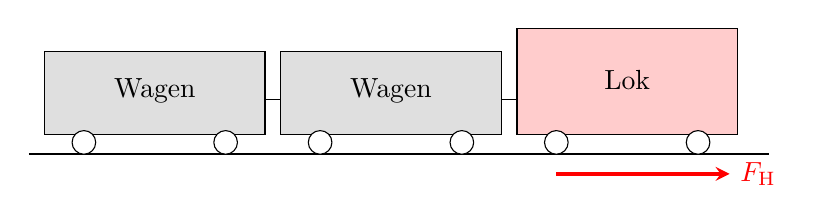
\begin{tikzpicture}[>=stealth]
 \draw[thick] (-5.2,0) -- (4.2,0);
 \draw[fill=gray!25] (-5,0.25) rectangle (-2.2,1.3);
 \draw[fill=gray!25] (-2,0.25) rectangle (0.8,1.3);
 \draw[fill=red!20] (1,0.25) rectangle (3.8,1.6);
 \draw (-2.2,0.7) -- (-2,0.7) (0.8,0.7) -- (1,0.7);
 \foreach \x in {-4.5,-2.7,-1.5,0.3,1.5,3.3} \draw[fill=white] (\x,0.15) circle (0.15);
 \node at (-3.6,0.8) {Wagen};
 \node at (-0.6,0.8) {Wagen};
 \node at (2.4,0.95) {Lok};
 \draw[->, very thick, red] (1.5,-0.25) -- ++(2.2,0) node[right] {$F_\mathrm{H}$};
\end{tikzpicture}
\end{center}

Die Räder rollen auf den Schienen, ohne zu rutschen. Antriebs- und Bremskraft sind deshalb Haftreibungskräfte zwischen Rad und Schiene. Für Stahl auf Stahl ist $\mu_\mathrm{H} = \muHO$ (FoTaBe S.~189).

\textbf{Beschleunigen:} Nur die Räder der Lokomotive werden angetrieben, die Antriebskraft ist höchstens $\mu_\mathrm{H}\,m_\mathrm{L}\,g$. Sie beschleunigt den ganzen Zug:
\begin{align}
 a &= \aZuF \\
   &= \frac{\muH\cdot\mLo\cdot\gE}{\mLo+\mWa} \\
   &= \aZu \approx \result{\aZuP{0}{2}}
\end{align}

\textbf{Bremsen:} Alle Räder werden gebremst, die Bremskraft ist höchstens $\mu_\mathrm{H}\left(m_\mathrm{L}+m_\mathrm{W}\right)g$, die Bremsverzögerung also
\begin{align}
 a_\mathrm{B} &= \aBrF = \muH\cdot\gE = \aBr
\end{align}
Die kürzeste Bremszeit ist
\begin{align}
 t_\mathrm{B} &= \frac{v_0}{a_\mathrm{B}} = \tBrF \\
   &= \frac{\vZu}{\muH\cdot\gE} \\
   &= \tBr \approx \result{\tBrP{0}{2}}
\end{align}
Die Geschwindigkeit nimmt gleichmässig ab, die mittlere Geschwindigkeit ist $v_0/2$. Der Bremsweg ist damit
\begin{align}
 s_\mathrm{B} &= \frac{v_0}{2}\cdot t_\mathrm{B} = \sBrF \\
   &= \frac{\vZu}{2}\cdot\tBr \\
   &= \sBr \approx \result{\sBrP{0}{2}}
\end{align}
Das sind theoretische Grenzwerte für saubere, trockene Schienen. Im Betrieb bremsen Güterzüge viel schwächer (etwa mit \aTyO), damit die Räder nicht blockieren und die Ladung nicht verrutscht.
